\documentclass[tikz,border=5pt]{standalone}
\usetikzlibrary{calc,positioning,intersections,shadows.blur,decorations.pathmorphing,patterns,shapes.callouts}

\definecolor{moonGray}{RGB}{180,180,180}
\definecolor{craterGray}{RGB}{120,120,120}
\definecolor{spaceBlue}{RGB}{10,10,40}
\definecolor{sunlight}{RGB}{255, 215, 0}
\definecolor{earthBlue}{RGB}{60,170,255}
\definecolor{earthGreen}{RGB}{40,140,60}

\begin{document}
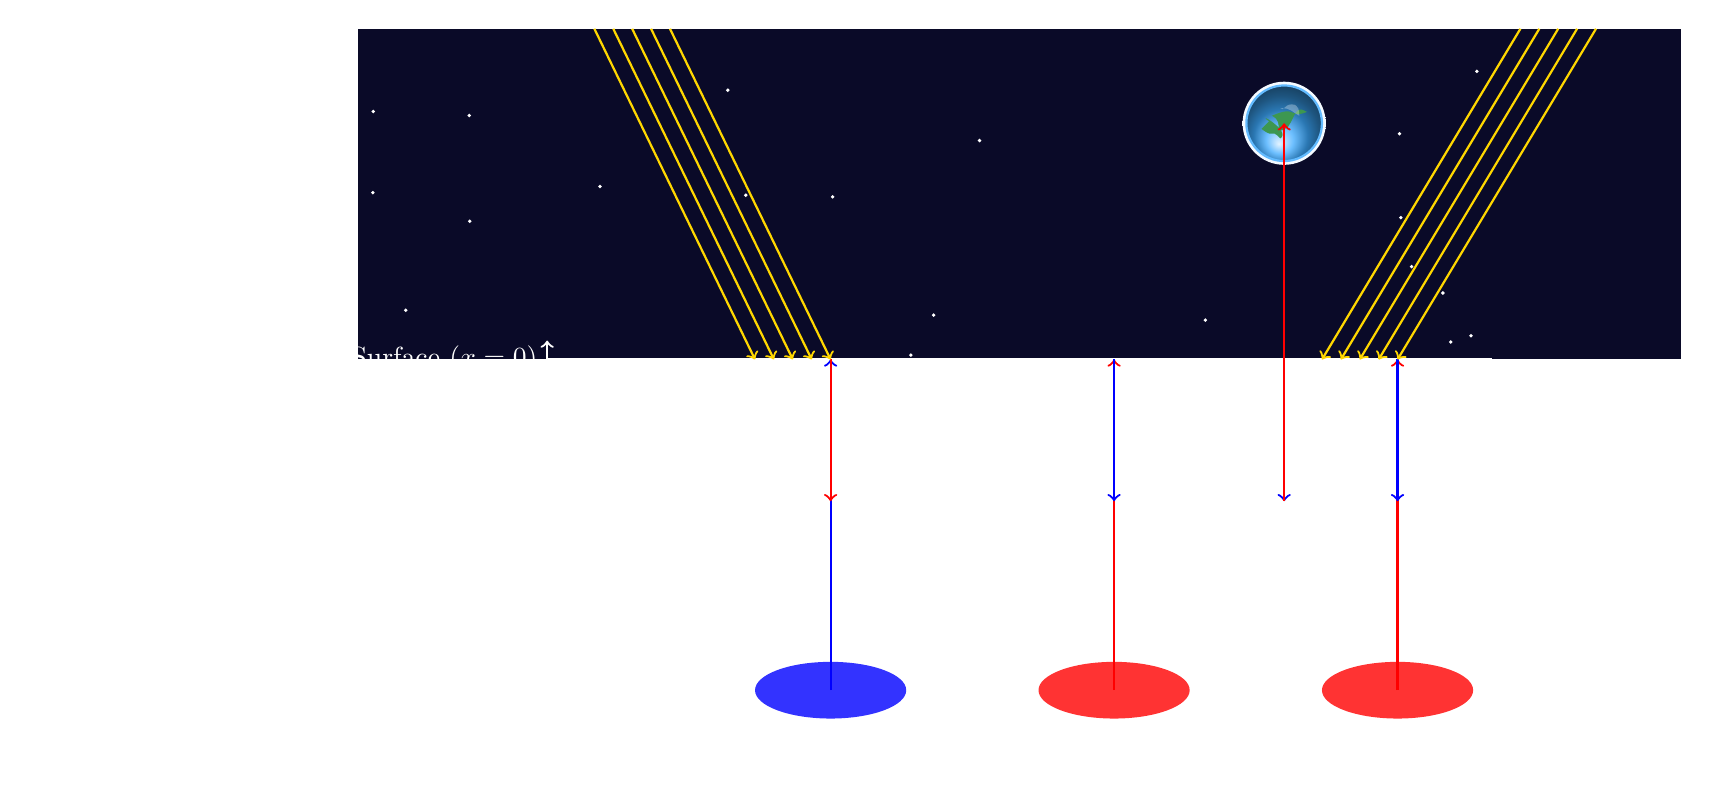
\begin{tikzpicture}[scale=1.2]

% Background (space) - with stars
\fill[spaceBlue] (-12,0) rectangle (2,3.5);
\foreach \i in {1,...,40}{
  \fill[white] (rand*8-8,rand*2+1.2) circle (0.02);
}

% Surface line
\draw[white,very thick] (-10,0) -- (0,0);
\node[white,anchor=east] at (-10,0) {Surface ($x=0$)};

% Vertical axis
\draw[->,white,thick] (-10,-4) -- (-10,0.2) node[midway,left] {$x$};
\node[white,anchor=north] at (-10,-4) {Deep Interior};

% Dotted vertical dividers with equal spacing
\foreach \x in {-7,-4,-1}
    \draw[white,dashed,thick] (\x,0) -- (\x,-4);

% Blue circle and arrow (left)
\fill[blue!80] (-7,-3.5) ellipse (0.8 and 0.3);
\draw[blue,thick,->] (-7,-3.5) -- (-7,0);

\draw[red,thick,->] (-7,0) -- (-7,-1.5);

% Red circles and arrows (middle and right) with equal spacing
\foreach \x in {-4,-1} {
    \fill[red!80] (\x,-3.5) ellipse (0.8 and 0.3);
    \draw[red,thick,->] (\x,-3.5) -- (\x,0);
    \draw[blue,thick,->] (\x,0) -- (\x,-1.5);
}

% Enhanced Earth with atmosphere and continents
\begin{scope}
% Atmosphere glow
\shade[inner color=earthBlue!30, outer color=earthBlue!5] (-2.2,2.5) circle (1.1*0.4);

% Main Earth body
\shade[ball color=earthBlue, shading angle=120] (-2.2,2.5) circle (0.4);

% Enhanced continents
\begin{scope}
  \clip (-2.2,2.5) circle (0.4);
  \fill[earthGreen!90] ($(-2.2,2.5)+(-0.13,0.08)$) 
        .. controls +(0.28,0.12) and +(-0.2,-0.08) .. ($(-2.2,2.5)+(0.24,0.12)$)
        .. controls +(-0.12,0.08) and +(0.08,0.12) .. ($(-2.2,2.5)+(0.04,-0.04)$)
        .. controls +(-0.2,-0.12) and +(0.16,-0.08) .. cycle;
  
  \fill[earthGreen!90] ($(-2.2,2.5)+(-0.24,-0.06)$) 
        .. controls +(0.16,-0.12) and +(-0.12,0.12) .. ($(-2.2,2.5)+(-0.04,-0.16)$)
        .. controls +(0.12,0.08) and +(-0.16,0.12) .. ($(-2.2,2.5)+(-0.16,0.02)$) -- cycle;
        
  % Cloud patterns
  \fill[white,opacity=0.3] ($(-2.2,2.5)+(-0.04,0.16)$) 
        .. controls +(0.12,0) and +(-0.08,0.04) .. ($(-2.2,2.5)+(0.16,0.08)$)
        .. controls +(0,0.04) and +(0.08,0) .. ($(-2.2,2.5)+(0.08,0.2)$)
        .. controls +(-0.08,0) and +(0.04,-0.04) .. cycle;
\end{scope}

\draw[thick,earthBlue!80] (-2.2,2.5) circle (0.4);
\end{scope}

% 5 parallel rays from top left hitting surface above left bubble (angled)
\foreach \i in {0,...,4} {
    \draw[sunlight,thick,->] (-9.5 + \i*0.2, 3.5) -- (-7.8 + \i*0.2, 0);
}

% 5 parallel rays from top right hitting surface above right bubble (symmetric angle)
\foreach \i in {0,...,4} {
    \draw[sunlight,thick,->] (0.3 + \i*0.2, 3.5) -- (-1.8 + \i*0.2, 0);
}

% Arrows showing flux at surface (blue down, red up)
\draw[blue,thick,->] (-2.2,0) -- (-2.2,-1.5);
\draw[red,thick,->] (-2.2,-1.5) -- (-2.2,2.5);

\end{tikzpicture}
\end{document}